\chapter{Software di benchmark}
\fancyhead[RO]{\bfseries Software di benchmark}
\section{Definizione del software di benchmark}
Per valutare la qualità dell'algoritmo si è rivelato utile sviluppare un software in grado di raccogliere informazioni sull'efficenza dell'algoritmo stesso in tutte le possibili combinazioni di punto di arrivo/punto di partenza in simulazioni di dimensioni fissate. 

In particolare sono stati osservati i casi peggiori, la media aritmetica dei casi, lo scarto quadratico medio, e i risultati ottenuti più frequentemente. Il software permette di testare qualsiasi algoritmo in grado di interfacciarsi con il sistema di gioco. 

NSi è ritenuto opportuno fare un confronto con un algoritmo greedy ottimo, ad informazione completa sugli stati del mondo. Il termine di paragone è quindi il rapporto tra i valori raccolti attraverso l'esecuzione dell'algoritmo ottimo e quelli ottenuti con l'esecuzione dell'algoritmo descritto, più questo si avvicina ad 1, più le prestazioni dell'algoritmo sviluppato si avvicinano a quelle dell'algoritmo ottimo. 
Il rapporto non sarà mai pari ad 1 a causa della differenza delle informazioni riguardo il mondo che i due agenti hanno, quindi la valutazione ha un carattere simbolico. Può però diventare interessante nel caso in cui vengano sviluppati altri algoritmi atti a risolvere la stessa problematica per un confronto con la stessa conoscenza del mondo.

\section{Parametri che influenzano la qualità del risultato}
Ci sono dei parametri che possono essere modificati influenzando i risultati. 

Il primo è il numero di volte in cui il Drone debba passare su uno stesso punto prima di decidere di cambiare strategia e riniziare con la calibrazione. Attraverso l'osservazione dei diversi casi si è notato che facilmente l'agente può trovarsi a passare due volte nello stesso punto durante la ricerca. Ad esempio nel caso si stia allontando dalla sorgente e ci sia bisogno di cambiare direzione. Considerando però dimensioni del mondo relativamente grandi, è probabile che incorrendo tre o più volte nello stesso punto si stia percorrendo un ciclo di movimenti. Questo in particolare nel caso in cui la dimensione del grafo che rappresenta il KB  sia controllata, quindi il numero di nodi memorizzati minore del numero di passi effettuati. Si è quindi impostato questo parametro in modo da cambiare strategia quando il Drone passa per la terza volta in uno stesso punto.

Il secondo parametro che preso in considerazione è il numero di passi in orrizontale e in verticale da far svolgere al Drone durante la calibrazione. Nel caso in cui venga svolto un solo passo per direzione, se l'obiettivo si trova su uno degli assi che incrociano il punto di partenza, l'agente si muoverà comunque in diagonale. Permettendo di fare due passi in orizzontale, due in verticale e uno verso il punto di partenza in diagonale, nel caso in cui l'obiettivo si trovi su uno degli assi che si incontrano nell'ultimo punto in cui ci si è spostati, il drone andrebbe direttamente nella direzione del punto di arrivo. Si è notato però che questo approccio non modifica significativamente i risultati nel caso di dimensioni del mondo relativamente grandi e ne peggiora la media nel caso di piccole dimensioni. Per questo è stato preferito far svolgere all'agente un solo passo per direzione.

Il terzo parametro è il limite alle dimensioni del grafo. È necessario che questo possa contenere almeno 4 elementi, per poter eseguire la calibrazione e le successive decisioni. Ogni altro nodo memorizzato è utile per il cambio strategia, permettendo di evitare di passare più di 3 volte sullo stesso punto. La necessità di cambiare strategia non si presenta nella media dei casi, ma in particolari situazioni, quindi impostare questo limite potrebbe peggiorare il caso peggiore, senza influenzare in maniera significativa la media dei risultati.
	
\section{Risultati}
La tecnica è pensata per lavorare in campo aperto, in assenza di ostacoli. L'algoritmo viene testato in un ampio numero di casi significativi.

Quelle che seguono sono le schermate della suite di benchmark, richiamata con 

\begin{verbatim} $ python curses_tests.py \end{verbatim}

per testare l'algoritmo su una matrice 20x20.

\begin{figure}[hb]
\center
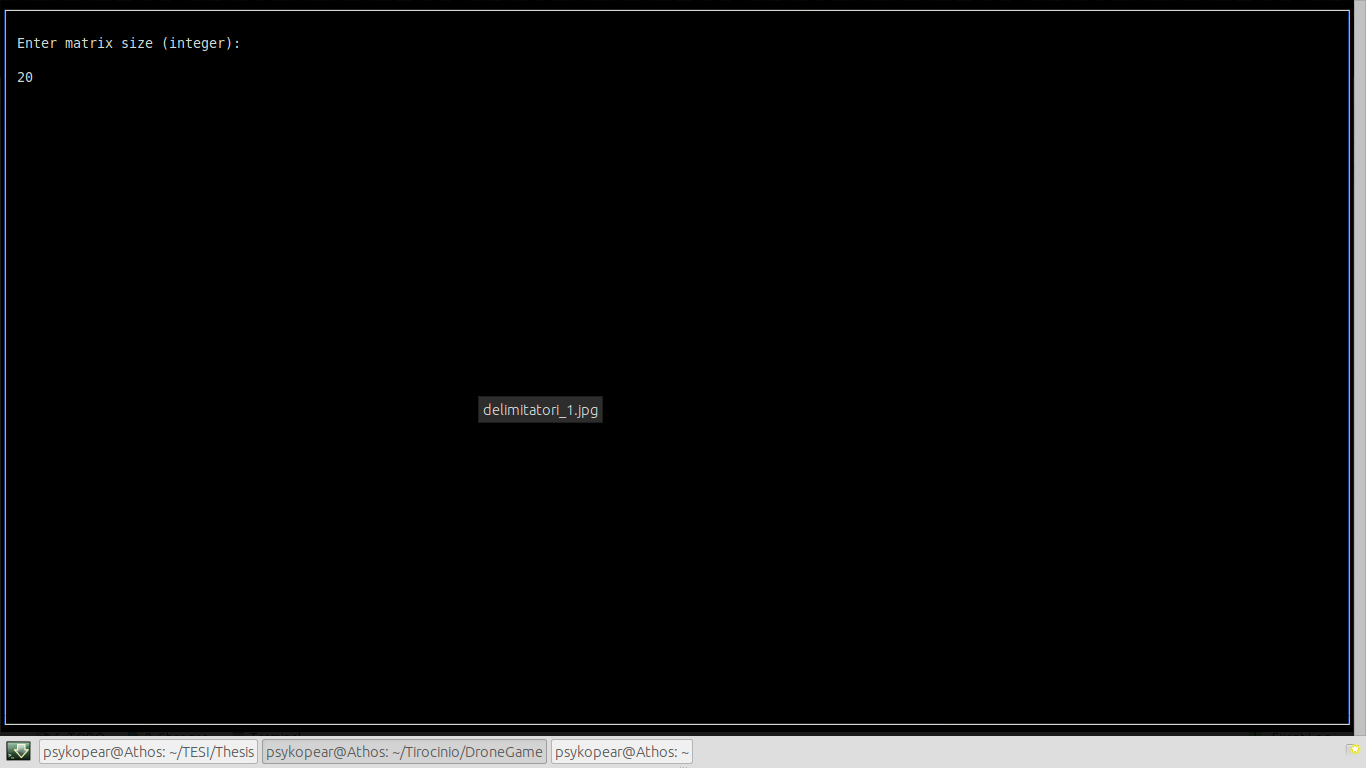
\includegraphics[width=\textwidth]{immagini/Test1-1.png}
\caption{Si inserisce la dimensione della matrice.}
\end{figure}

\begin{figure}[hb]
\center
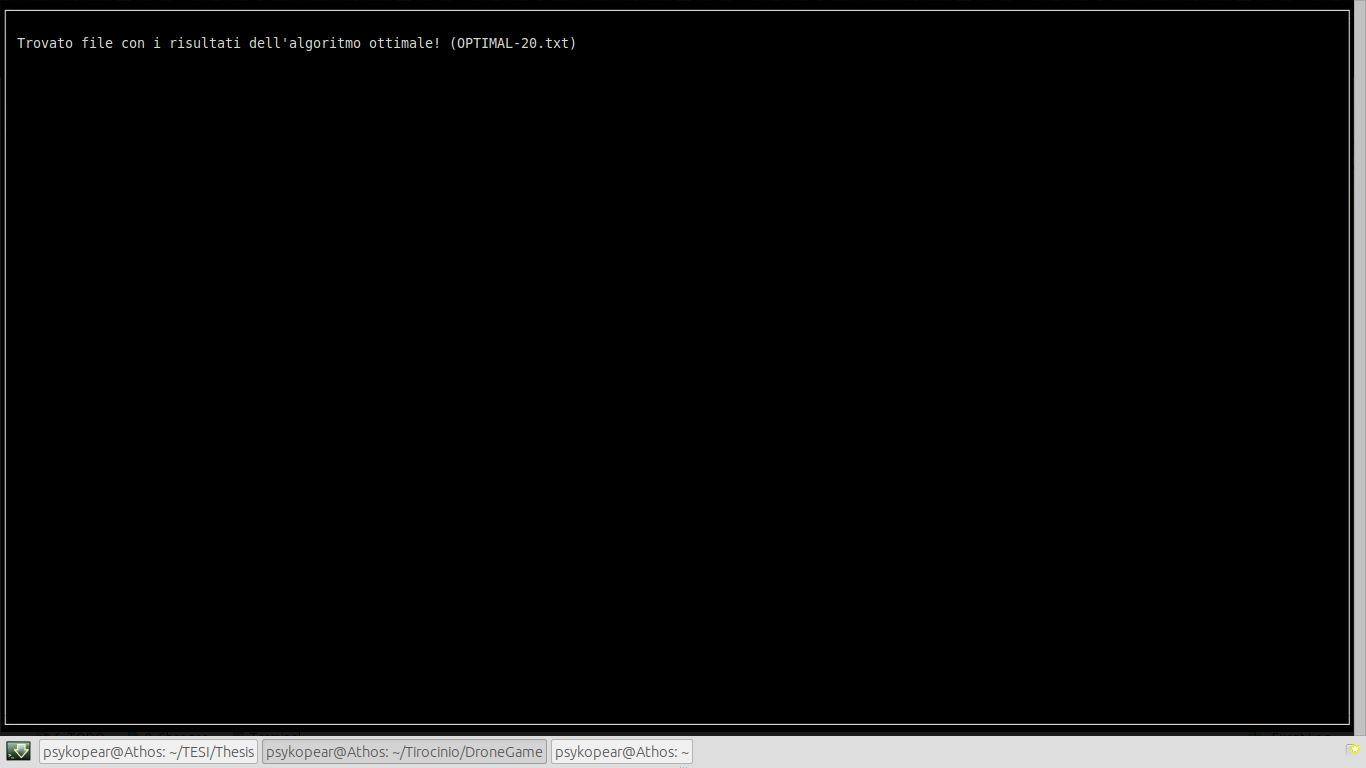
\includegraphics[width=\textwidth]{immagini/test2.png}
\caption{Se nella cartella è presente un file con i risultati dell'algoritmo ottimale, viene utilizzato questo invece di rifare i calcoli.}
\end{figure}

\begin{figure}[hb]
\center
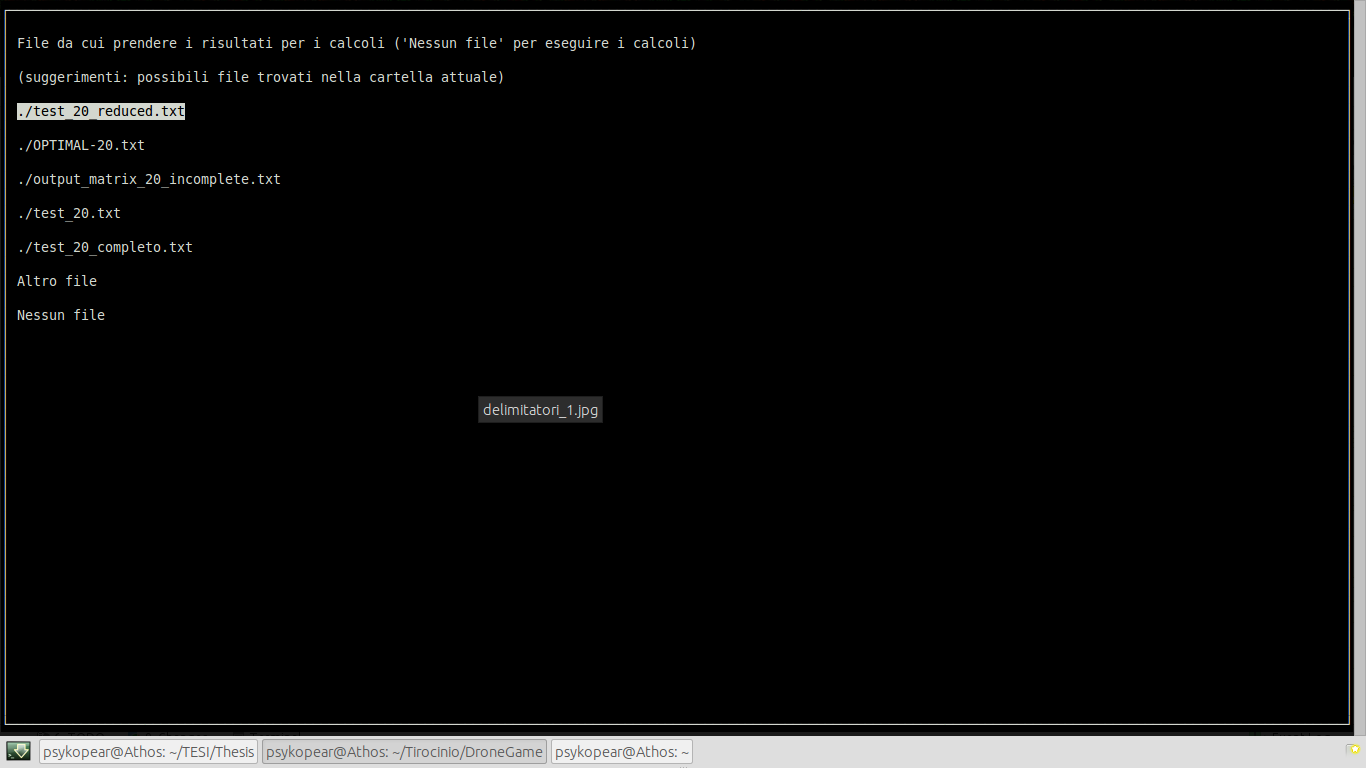
\includegraphics[width=\textwidth]{immagini/test3.png}
\caption{Si possono prelevare i dati anche per l'algoritmo in test, se questi sono stati salvati su un file, evitando di eseguire i calcoli.}
\end{figure}

\begin{figure}[hb]
\center
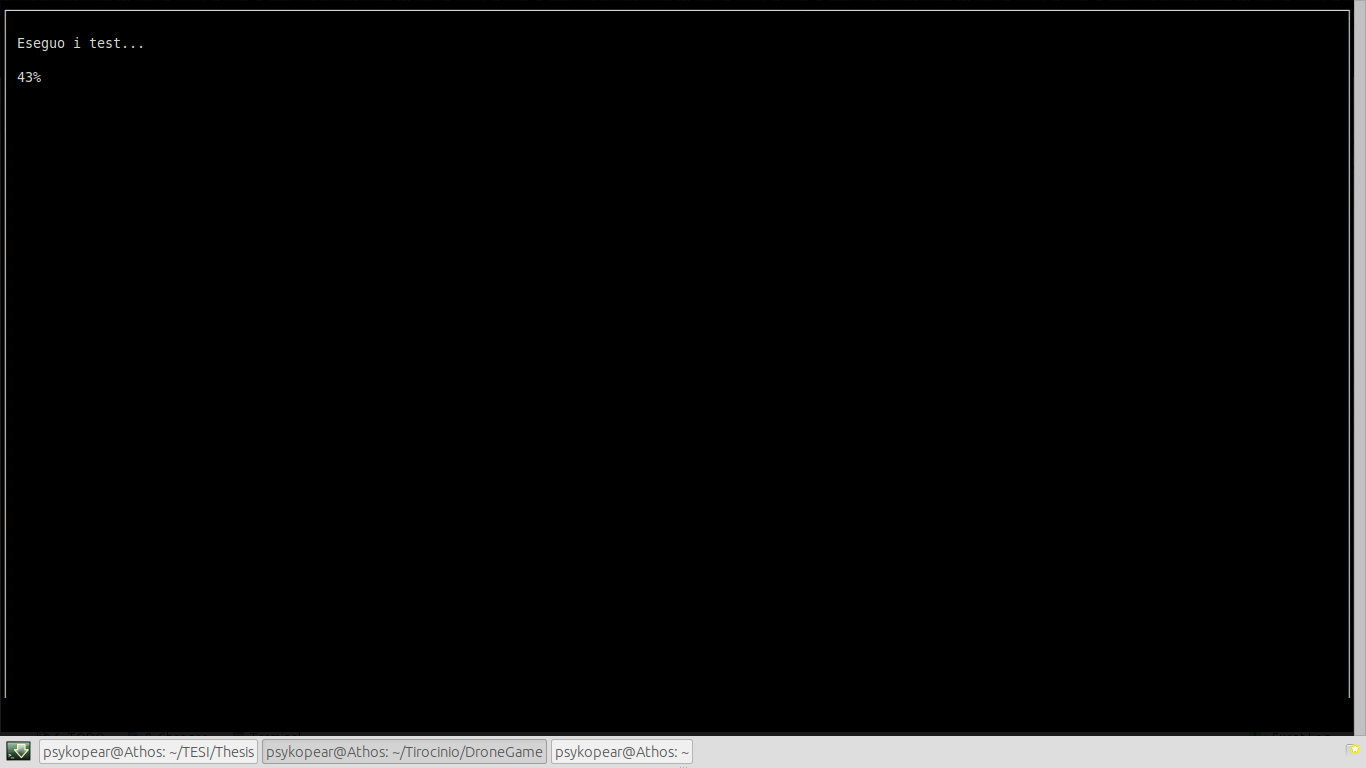
\includegraphics[width=\textwidth]{immagini/test5.png}
\caption{Test in esecuzione...}
\end{figure}

\begin{figure}[hb]
\center
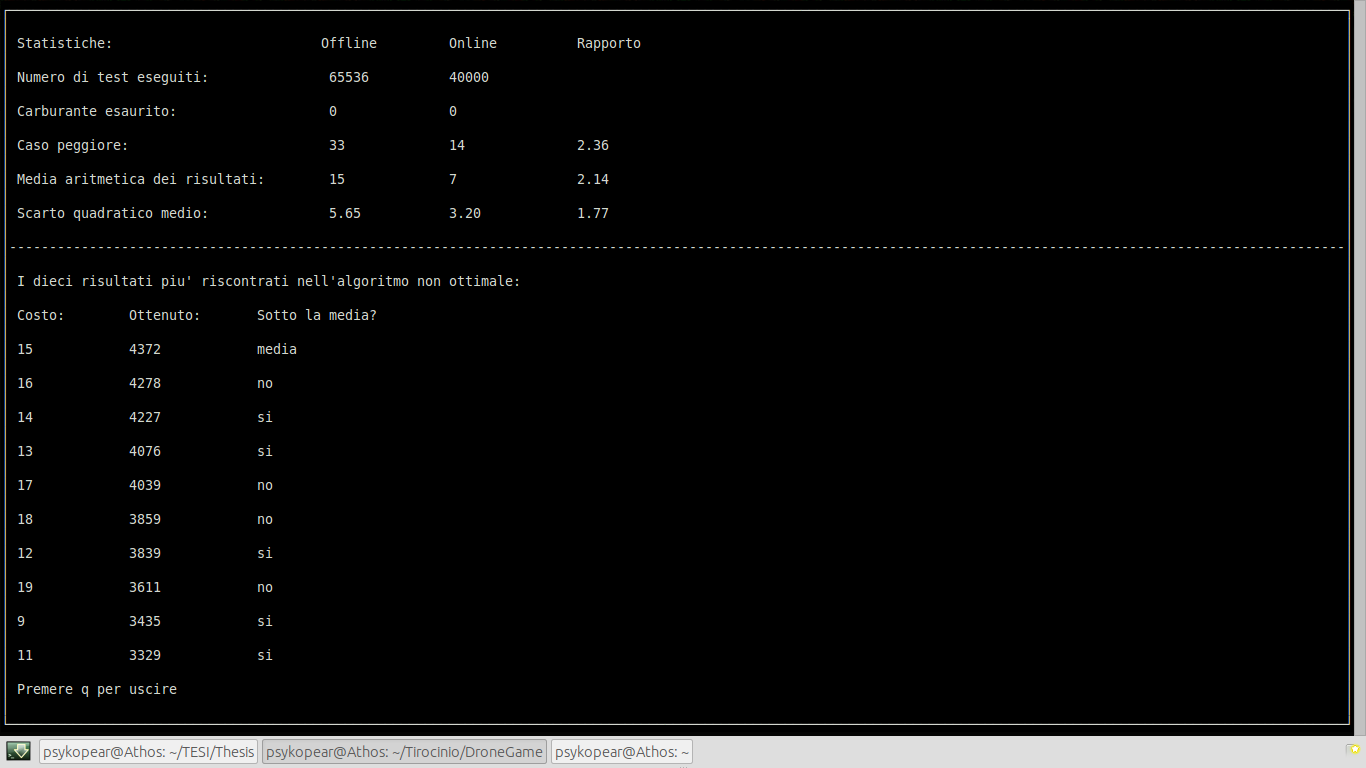
\includegraphics[width=\textwidth]{immagini/Results.png}
\caption{Vengono visualizzati a schermo i risultati ottenuti}
\end{figure}